% document type
\documentclass[a4paper,12pt]{article}
% show name on citation
\usepackage[round]{natbib}
\bibliographystyle{plainnat}
\usepackage[utf8]{inputenc}
\usepackage[T1]{fontenc}
% language
\usepackage[portuguese]{babel}
% font family
\usepackage{helvet}
\renewcommand{\familydefault}{\sfdefault}
% line spacing
\linespread{1.5} 
% always indent paragraph
\usepackage{indentfirst}
% footnote always at end of page
\usepackage[bottom]{footmisc}
% clickable links
\usepackage{hyperref}
%define colors
\usepackage[dvipsnames]{xcolor}
\newcommand\myshade{}
\colorlet{mylinkcolor}{black}
\colorlet{mycitecolor}{MidnightBlue}
\colorlet{myurlcolor}{blue}
% set color for each type of link
\hypersetup{
  colorlinks = true,
  citecolor  = mycitecolor!\myshade!black,
  linkcolor  = mylinkcolor!\myshade!black,
  urlcolor   = myurlcolor!\myshade!black,
}

% package to include images
\usepackage{float}
\usepackage[pass]{geometry}
\usepackage{graphicx}
\graphicspath{{images/}}
% title for table of contents
\addto\captionsportuguese{
  \renewcommand{\contentsname}
    {Sumário}
}
% table style
\usepackage{longtable}
\usepackage{multirow}
\usepackage[table]{colortbl}

% word breaks
\usepackage{hyphenat}
\hyphenation{Im-ple-men-tação}


\title{}
\author{Gabriel R. Zsigmond}
\date{30 setembro 2020}

\begin{document}
  \newgeometry{margin=80pt}
  \begin{titlepage}
    \begin{center}
        \vspace*{1cm}
        \LARGE
        \textbf{COMPUTADORES CLÁSSICOS E QUÂNTICOS:}
        
        \vspace{0.5cm}
        \large
        ESTUDOS, IMPLEMENTAÇÕES E IMPACTOS SOCIAIS
        
        \vspace{1.5cm}
        
        \textbf{Gabriel R. Zsigmond}
        \vfill
        
        INICIAÇÃO CIENTÍFICA
        
        \vspace{0.8cm}
        
        
\includegraphics[width=0.4\textwidth]{espm.png}\\
        \large
        ESCOLA SUPERIOR DE PROPAGANDA E MARKETING\\
        Sistemas de Informação em Comunicação e Gestão\\
        Brasil\\
        30 de abril de 2021\\
        
    \end{center}
\end{titlepage}
  \begin{titlepage}

    \begin{center}
        
        \textbf{Gabriel R. Zsigmond}
        
        \vspace{3cm}
        
        \LARGE
        \textbf{COMPUTADORES CLÁSSICOS E QUÂNTICOS:}
        
        \vspace{0.5cm}
        \large
        ESTUDOS, IMPLEMENTAÇÕES E IMPACTOS SOCIAIS
        
        \vspace{3.5cm}
        
        \begin{flushright}
        \begin{minipage}{10cm}
        Projeto de Iniciação Científica para a Escola Superior de Propaganda e Marketing, sob a orientação do Professor Doutor Humberto Sandmann.\linebreak[3]
        
        Orientador: Prof. Dr. Humberto Sandmann
        \end{minipage}
        \end{flushright}
        \vfill
        
        Brasil\\
        05 de maio de 2020\\
        
    \end{center}

\end{titlepage}
  \thispagestyle{plain}
\begin{center}
    \Large
    \textbf{ESTUDOS, IMPLEMENTAÇÕES E IMPACTOS SOCIAIS:}
    
    \vspace{0.4cm}
    \large
    ESTUDOS, IMPLEMENTAÇÕES E IMPACTOS SOCIAIS
    
    \vspace{0.4cm}
    \textbf{Gabriel R. Zsigmond}
    
    \vspace{0.9cm}
    \textbf{Resumo}
\end{center}
O presente projeto, "Computadores Clássicos e Quânticos: Estudos, Implementação, Simuladores e Impactos Sociais", se propõe a estudar a história do computador e sua evolução. A mais recente inovação na área é a computação quântica, que certamente, inaugura a próxima geração de computadores. A computação quântica muda toda uma arquitetura na forma de computação, permitindo que os novos computadores sejam exponencialmente mais eficientes quando comparados aos mais modernos da atualidade. O projeto se propõe a entender e prototipar um computador tradicional de 8 bits em hardware, usando apenas portas lógicas simples, a fim de ilustrar, de forma clara, o funcionamento de um computador tradicional. Também, esse projeto busca entender e estimar as consequências sociais que os avanços da tecnologia e o desenvolvimento da computação quântica pode gerar. Entende-se que para essa análise, se faz necessário, inicialmente, uma ampla revisão bibliográfica, a fim de comparar esses dois tipos de computadores. Para ilustrar esta, será desenvolvida uma aplicação web que simula um computador tradicional e um computador quântico executando o mesmo algoritmo. É esperado que ao final do projeto, esse estudo traga um amplo e aprofundado conhecimento da área, além de, uma contribuição em relação ao impacto social do uso computação da quântica.
  \newpage
  \tableofcontents
  \newpage
  \listoftables
  \newpage
  \listoffigures
  \newpage
  \section{Introdução} 
\subsection{Definição justificada dos objetivos e da sua relevância}
A palavra “computador” é usada desde o século XVII, tendo a sua primeira referência escrita datada de 1613. No entanto, por muito tempo “computador” não tinha o mesmo significado que leva hoje, sendo utilizada, até a década de 1940, como nome da profissão de alguém que calcula, segundo o dicionário Michaelis: “Aquele ou aquilo que calcula baseado em valores digitais; calculador, calculista”. \cite{4}

Tendo em vista o antigo significado da palavra “computador”, pode-se questionar sobre como passamos a utilizar de uma palavra usada para se referir à pessoas, para mera maquinas. A fim de responder essa pergunta, recuperaremos a origem dos computadores. Pode parecer uma pergunta simplista que não precisa ser respondida, porém, é uma pergunta para a qual muitas pessoas não sabem a verdadeira resposta. Computadores existem há muito mais tempo que o transistor – dispositivo semicondutor usado para amplificar ou alternar sinais eletrônicos e eletricidade. – na forma mecânica e teórica. A definição real de um computador foi elaborada por Alan Turing (Reino Unido, 1912-1954), um matemático, lógico, criptógrafo e herói de guerra que se preocupava exatamente com a questão relacionada ao que era computável e o que não era. Ele foi responsável por elaborar a definição do computador, descrevendo a Maquina de Turing, trabalho publicado em 1937 que deu origem aos computadores e celulares que você, leitor, pode estar usando para ler o presente trabalho.

A Maquina de Turing, considerado o modelo mais poderoso computador, é similar a um automato finito\footnote{Um sub-tópico da Ciência da computação teórica, também chamado máquina de estados finita determinística — é uma máquina de estados finita que aceita ou rejeita cadeias de símbolos gerando um único ramo de computação para cada cadeia de entrada.}, porém com uma mémoria ilimitada e irrestrita, constituindo um modelo mais exato de um computador de forma geral. Esta é composta por três principais componentes: fita infinita; processador; máquina de estado finito. 

A fita infinita é dividida em células, cada uma contendo um simbolo de um alfabeto finito. O processador é responsável por se deslocar para a direita ou esquerda e efetuar a leitura ou escrita em uma célula. Assim, a explicação adaptada do material do Fabio Gagliardi Cozman \cite{7}, ilustra seu funcionamento da seguinte forma:
\begin{enumerate}
  \item Inicialmente a fita contém somente a cadeia de entrada, disposta no “meio”\footnote{Meio é algo abstrato nesse sentido pois não existe meio de um valor infinito} da fita , com o processador posicionado no início da cadeia (o resto está em branco);
  \item Para armazenar algo, a máquina escreve na fita;
  \item O processador pode ser movido livremente para a esquerda ou direita, afim de ler ou escrever valores em qualquer célula;
  \item As saídas aceita e rejeita são obtidas ao entrar nos estados de aceitação e rejeição;
  \item Se não entrar em um estado de aceitação ou rejeição, continuará sua computação para sempre (loop infinito).
\end{enumerate}

Já o primeiro computador digital eletrônico de grande escala, foi criado em fevereiro de 1946 por cientistas norte-americanos, John Presper Eckert e John W. Mauchly, da Electronic Control Company . No final de sua operação em 1956, o ENIAC (Electrical Numerical Integrator and Calculator), continha 20.000 tubos de vácuo 7.200 diodos de cristal 1.500 relés 70.000 resistores 10.000 capacitores e aproximadamente 5.000.000 juntas soldadas à mão. Ele pesava mais de 27 toneladas, tinha aproximadamente 2,4m * 0,9m * 30m de tamanho, ocupava 167 m2 e consumia 150 kW de eletricidade. \cite{2}

A partir do ENIAC, as possibiliades tecnologicas tomaram uma nova proporção. Em 1969, apenas 13 anos após o desligamento do primeiro computador digital eletronico, o computador de bordo da Apollo 11, missão que levou o homem a lua, tinha 32.768 bits [para uma explicação elaborada sobre bits refira-se ao cápitilo \ref{bits} pagina \pageref{bits}] de RAM, o suficiente para armazenar apenas um texto não formatado, com cerca de 2.000 palavras. Em 2018, o iPhone XS, com 4GB de RAM (ou 34.359.738.368 bits), tem cerca de 1 milhão de vezes mais memória que o Apollo Guinche Computer. \cite{5}

(falar da Spacex e falcon9 e CRS-12 Dragon 2020)

Durante o século XX, além do aumento de poder computacional dos dispositivos, outro fator impactante foi a refatoração de seus tamanhos. Assim, com tecnologias wearables\footnote{A tecnologia em questão não somente pode ser usada como uma peça de roupa ou um acessório, como também tem que possuir características que a conectem a outros aparelhos ou à internet.}, os computadores se tornam ativamente presentes no cotidiano.

Levando em consideração o rápido avanço e desenvolvimento computacional, mencionados anteriormente, entende-se que os computadores agregam à sociedade, seja facilitando a comunicação e o compartilhamento de conhecimentos, como em outros aspectos. No entanto, a agilidade pela qual se deu tais transformações da tecnologia da computação, também gera grandes expectativas e incertezas sobre o que ainda está por vir, tanto nas questões de mudanças tecnológicas quanto nos impactos relevantes na sociedade.

Tendo em vista a incerteza sobre o futuro da computação em relação aos proximos grandes avanços, nessa pesquisa serão estudados os conceitos da física clássica e da física quântica aplicados à computação, além disso, será estudado os princípios de criptografia\footnote{Criptografia é um sistema de algoritmos matemáticos que codificam dados para que só o destinatário possa ler.}. Assim, a presente pesquisa irá prototipar um computador clássico de 8 bits em hardware usando apenas portas lógicas simples, dessa forma, ilustrando claramente o seu funcionamento. Junto a isso também será desenvolvida uma aplicação web que ilustre o funcionamento de um processador quântico. Ao final, conceitos de criptografia serão ultilizados para exemplificar possíveis mudanças sociais que os próximos avanços tecnologicos podem gerar.

\subsection{Metodologia a ser empregada}
Para a realização da pesquisa de iniciação cientifica, é indispensavel o uso de pesquisa bibliográfica, assim recuperando conhecimento científico acumulado sobre o assunto. Segundo Telma Cristiane Sasso de Lima, o conhecimento da realidade não é apenas a simples transposição dessa realidade para o pensamento, pelo contrário, consiste na reflexão crítica que se dá a partir de um conhecimento acumulado e que irá gerar uma síntese, o concreto pensado \cite{1}. E também a utilização do processo cientifico para a elaboração e efetivação do projeto em si. Ambas metodologias citadas acima, são cruciais para o desenvolvimento do relatório final na área de pesquisa em computação, já que na grande parte dos estudos científicos, a utilização do processo cientifico é frequentemente utilizada para um maior entendimento da obra e a construção do projeto se tornar mais facilmente executável.

Para o desenvolvimento da entrega do protótipo, computador de 8-bits, e para o simulador do computador quântico web, a principal metodologia utilizada será Project Based Learnig (PBL). De acordo com  David Van Andel, o PBL envolve os alunos em um processo rigoroso de investigação, onde eles fazem perguntas, encontram recursos e aplicam informações para resolver problemas do mundo real \cite{3}. Assim, assumisse que esta é a melhor metodologia para desenvolver um protótipo físico de um computador e programar um site.

\newpage
  \section{Metodologia empregada}
\label{methodologies}
Para a realização da presente pesquisa de iniciação científica, foi indispensável a realização de uma revisão bibliográfica, afim de recuperar e aprofundar o conhecimento científico já produzido, assim bem como, se interar do estado da arte na área. Segundo Telma Cristiane Sasso de Lima, o conhecimento da realidade não é apenas a simples transposição dessa realidade para o pensamento, mas sim a reflexão crítica, que se dá a partir de um conhecimento acumulado que irá gerar uma síntese, o concreto pensado \cite{1}. E também a utilização do processo científico para a elaboração e efetivação do projeto em si. Ambas metodologias citadas acima são cruciais para o desenvolvimento do relatório final na área de pesquisa em computação, já que em grande parte dos estudos, a utilização do processo científico é frequentemente utilizada para um maior entendimento da obra e para que a construção do projeto possa se tornar mais facilmente executável.

Assim, para o desenvolvimento da entrega do protótipo — computador de 8-bits — e para o simulador do computador quântico web, a principal metodologia utilizada será Project Based Learnig (PBL). De acordo com David Van Andel, o PBL envolve os alunos em um processo rigoroso de investigação, onde eles fazem perguntas, encontram recursos e aplicam informações para resolver problemas do mundo real \cite{3}. Entende-se que esta é a melhor metodologia para desenvolver um protótipo físico de um computador e programar um site.

Nos dois capítulos a seguir, \ref{classic_comp} e \ref{quantum_comp}, respectivamente Computação Clássica e Computação Quântica são apresentadas em uma curta revisão bibliográfica 

\newpage
  \section{Computação Clássica} 
Entende-se a importância de se compreender a origem e o desenvolvimento da computação clássica para o desenrolar da pesquisa, o que será apresentado em meio a este capítulo.

A computação clássica consiste em computadores que dependem da física clássica para operar. Estes são os computadores tradicionais que usamos em nosso dia-a-dia – seja eles Apple, Samsung, Dell ou qualquer outro –, também classificados como computadores binários, pois processam as instruções a partir de números binários, compostos apenas pelos símbolos “1” e “0”, ligado e desligado, respectivamente. Assim, julga-se importante e de larga relevância ao tema compreender essa representação numérica. 

Números binários ou números em base 2 são compostos por apenas dois dígitos, [0...1]. Dessa forma, seu funcionamento é similar ao sistema decimal, ou base 10, que são compostos por dez dígitos, [0...9]. No sistema decimal, é simples contar até nove, porém não existe um simbolo ou dígito para representar o número dez, sendo então representado por dois dígitos, “10”, sendo uma simples lógica de posicionamento. Mais uma vez, após o número “99”, é necessário utilizar da mesma regra para representar o número cem, “100”. Já em base 2, o número zero é representado pelo simbolo ``0'', e o número um por ``1''. O mesmo dilema é enfrentado ao chegar no próximo valor: dois. E então é usada a mesma lógica de posicionamento, em base dois. Desta forma, o número dois é representado por “10”, o três por “11”, quatro por “100” e assim por diante. Portanto, números binários podem se tornar longos e compostos por muitos dígitos que levam o nome de bits. \cite{6} É com base nos \label{bits}bits\footnote{A menor unidade de informação que pode ser armazenada ou transmitida na comunicação de dados.} ligados e desligados que o computador baseia a sua linguagem. Para transforma-lo em base dez é preciso avaliar o valor de cada bit de acordo com a sua posição. 

Exemplo: número binário $1011$:

\[ 1011(b) = 1*2^3 + 0*2^2 + 1*2^1 + 1*2^0\]
\[ = 8 + 0 + 2 + 1 = 11(decimal)\]

O peso de cada bit de um número binário depende da sua posição relativa ao número completo, sempre partindo da direita para a esquerda.

\begin{itemize}
  \item O peso do primeiro bit é $bit * 2^0$
  \item O peso do segundo bit é $bit * 2^1$
  \item O peso do terceiro bit é $bit * 2^2$
  \item O peso do quarto bit é $bit * 2^3$
\end{itemize}

A formúla ilustrada acima, pode ser exemplificada em uma fórmula genérica: 

\[= nth\: bit * 2^{n-1}\]

É possível notar que a regra para números binários, se repete para números em base 10.

Exemplo: número decimal $4392$:
\begin{itemize}
  \item O peso do primeiro bit é $2 * 10^0$
  \item O peso do segundo bit é $9 * 10^1$
  \item O peso do terceiro bit é $3 * 10^2$
  \item O peso do quarto bit é $4 * 10^3$
\end{itemize}
\[ 4392 = 4*10^3 + 3*10^2 + 9*10^1 + 2*10^0\]
\[= nth\: bit * 10^{n-1}\]

Essa regra se mantem verdadeira para qualquer base númerica.

\[= nth\: bit * (base)^{n-1}\]

Ao decorrer do texto serão referidos números em base 2, 10 e 16. 

\subsection{A computação clássica e sua evolução}
Alan Turing, matemático inglês, cientista da computação, lógico, criptoanalista, filósofo e biólogo teórico, publicou o artigo “On Computable Numbers with an Application to the Entscheidungs-problem” \cite{8} em 12 de novembro de 1937, artigo que viria a formar a teoria básica da computabilidade por várias décadas.

O mecanismo abstrato descrito no artigo de Turing fornece os conceitos fundamentais de computadores que outros engenheiros conceberam posteriormente. Na sua essência, uma Máquina de Turing é um dispositivo que manipula símbolos em uma tira de fita de acordo com uma tabela de regras. O cientista forneceu a formalização dos conceitos de “algoritmo” e “computação” na infância da ciência da computação. Apesar de sua simplicidade, uma Máquina de Turing pode ser adaptada para simular a lógica de qualquer algoritmo de computador e é útil para explicar as funções de uma CPU.

Apesar dos computadores clássicos serem atualmente descritos como tendo a chamada arquitetura de Von Neumann, acredita-se que o idealizador dessa arquitetura partiu dos modelos matemáticos desenvolvidos por Alan Turing, que incluia o conceito de programa armazenado, originado a partir da construção da Maquina de Turing. Conceito, também encontrado no projeto EDVAC de Von Neumann \cite{9}, que possibilita o armazenamento de instruções e dados na mesma memória, permitindo a manipulação de programas como dados, que se constitui como característica definidora do computador clássico. Assim, pode-se alegar que Turing é o pai do computador já que suas publicações antecedem a arquitetura de Von Neumann, além de existirem razões para se acreditar que este último conhecia os resultados do trabalho de Alan Turing \cite{10}, que podem ter inspirado as suas criações. Outro fator que corrobora para este entendimento, é que Turing foi o primeiro a explorar a idéia de uma máquina de uso geral por meio de sua noção de máquina universal – que constitui a base do computador clássico ao possibilitar o funcionamento da CPU em conjunto com a memória RAM. Ainda, tendo em vista as contribuições do matemático para a construção de uma classe importante de dispositivos de computação, o Bombe – um dispositivo eletromecânico usado pelos criptologistas britânicos para ajudar a decifrar as mensagens secretas criptografadas pela máquina alemã Enigma durante a Segunda Guerra Mundial – e posteriormente o seu design do ACE (Automatic Computing Engine), fica evidente as contribuições de Alan Turing para a invenção do computador moderno. A partir da fala de Turing abaixo, pode-se identificar o ACE como um tipo de realização física da máquina universal.

\textit{
  ``Some years ago I was researching on what might now be described as an investigation of the theoretical possibilities and limitations of digital computing machines. […] Machines such as the ACE may be regarded as practical versions of this same type of machine.'' \cite{11}
}

Por fim, entende-se que baseado na teoria da máquina de Turing, o físico e matemático John von Neumann desenvolveu uma arquitetura capaz de executar as seguintes tarefas.

\vspace{1cm}
\begin{figure}[H] \centering 
  \makebox[\textwidth][c]{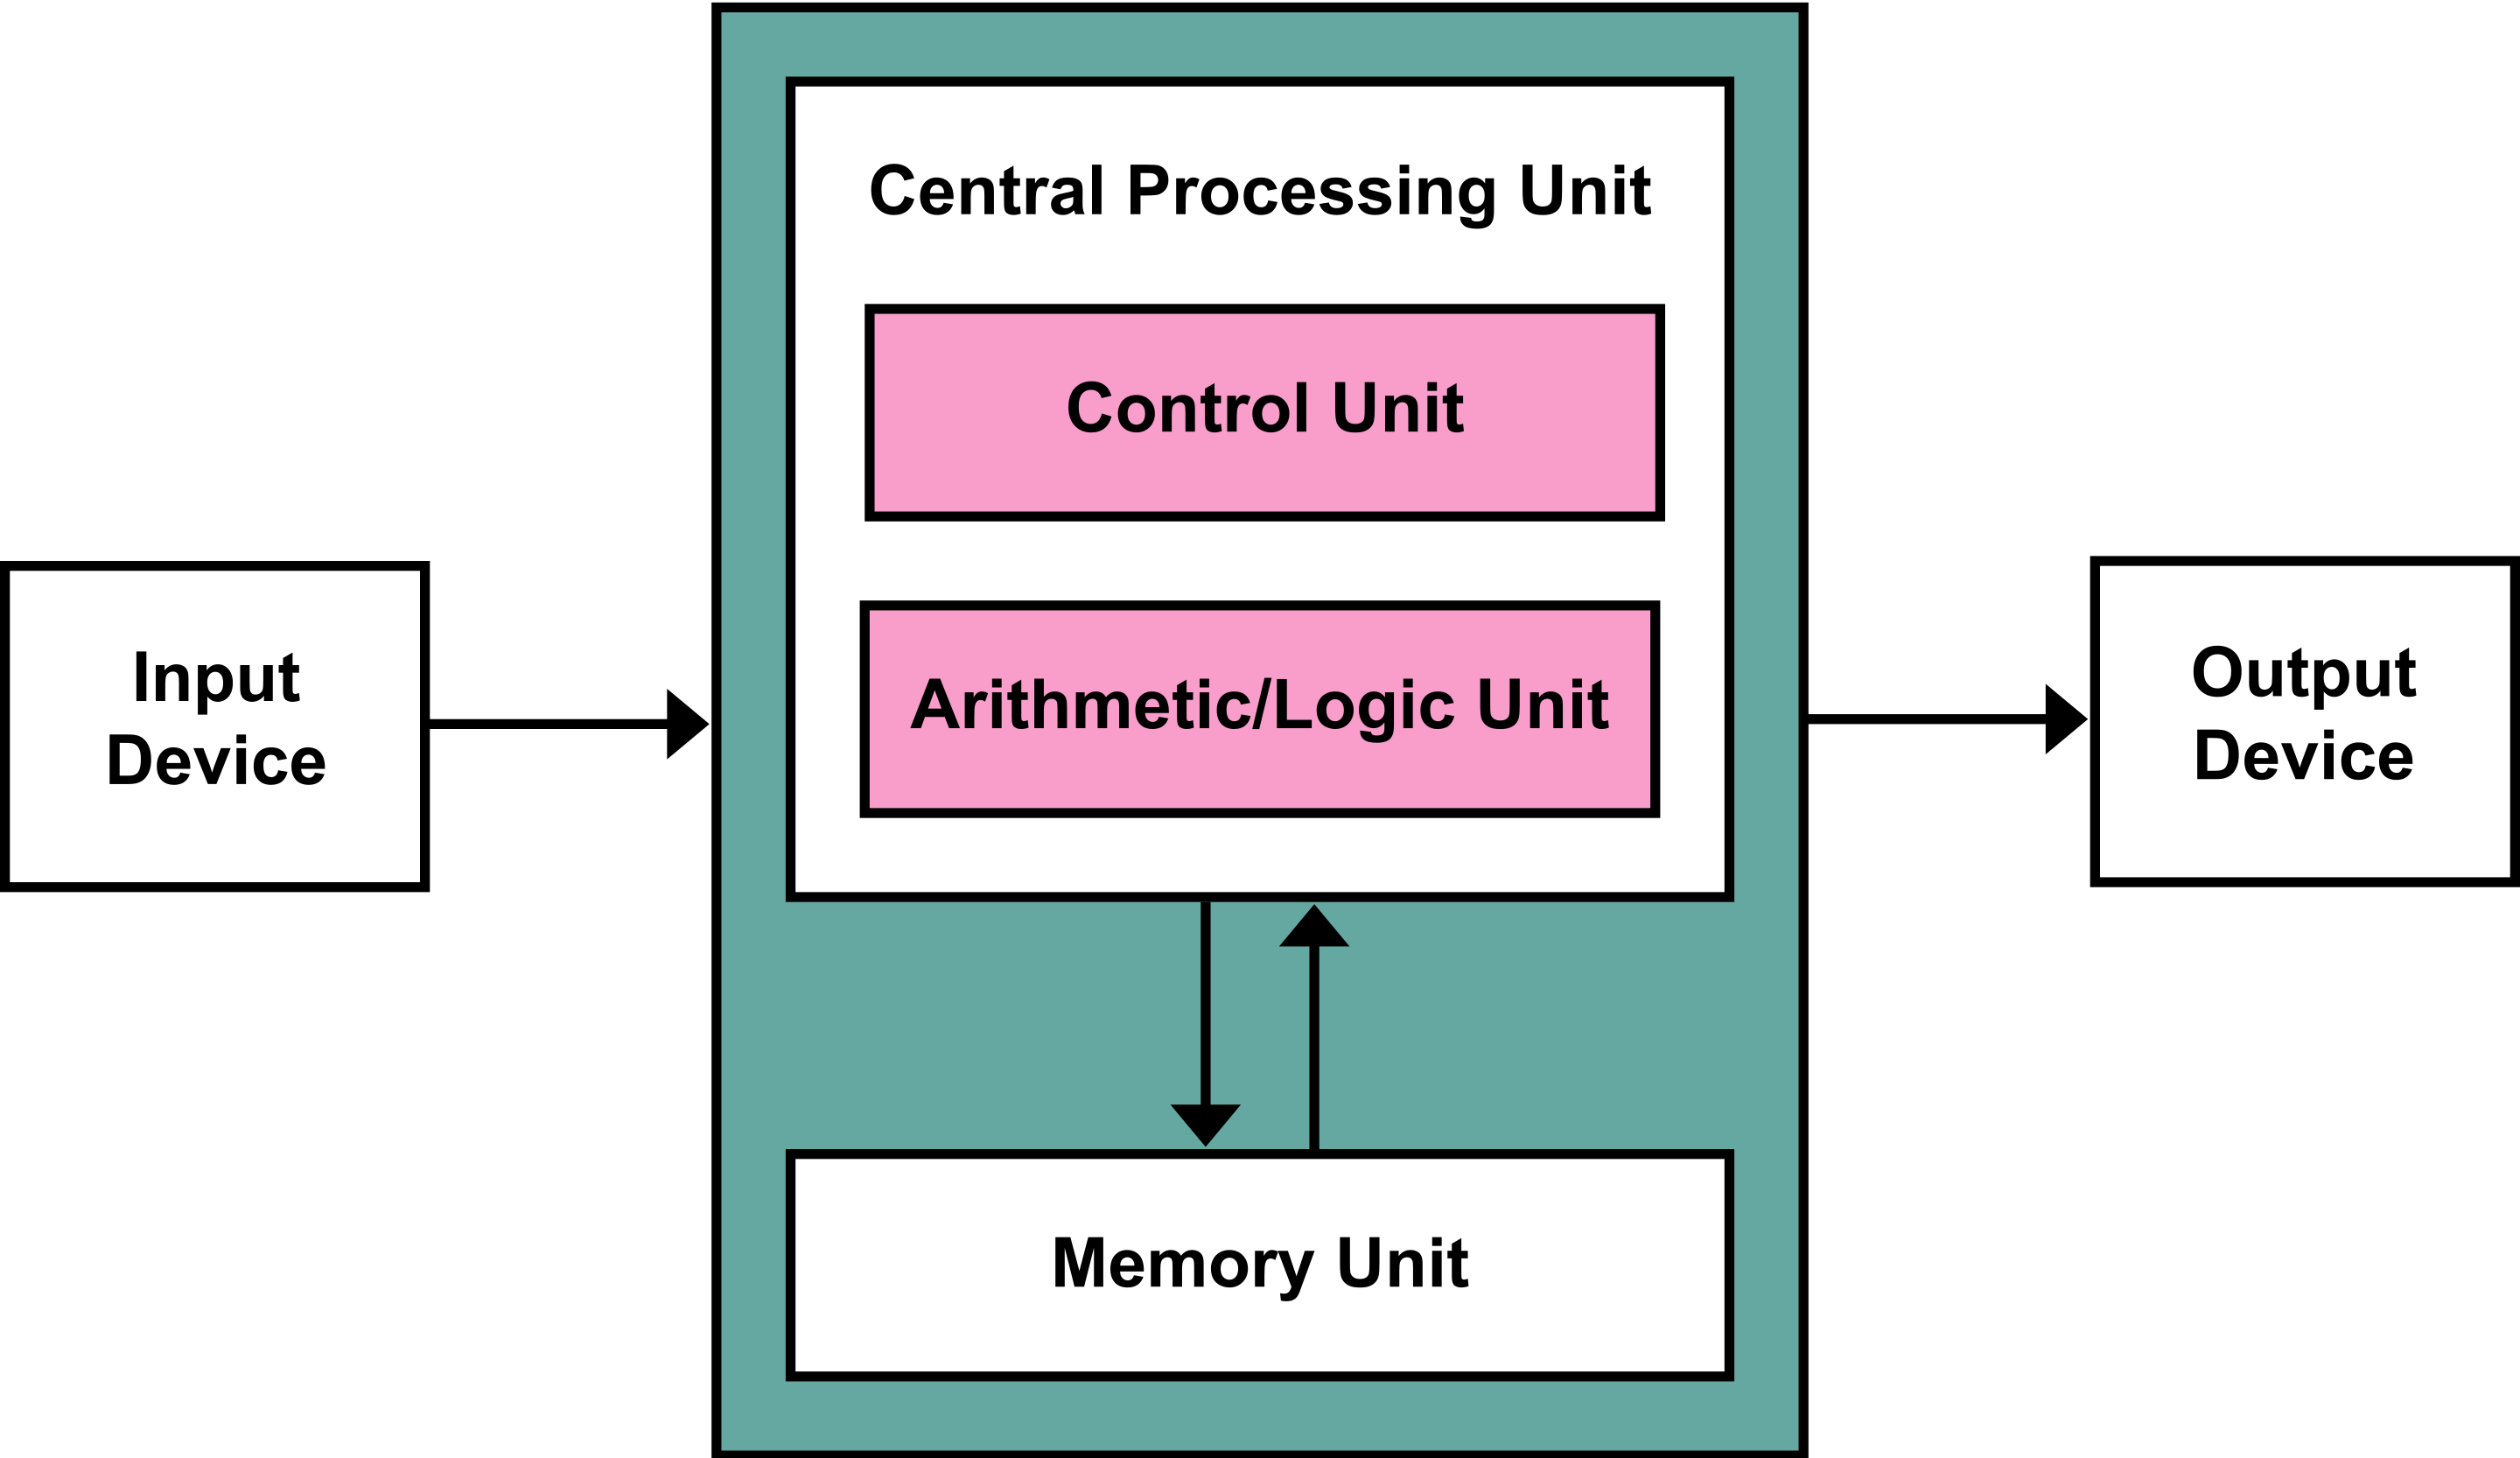
\includegraphics[width=0.8\textwidth]{von_neumann_architecture}}
  \caption{\label{fig:1} Diagrama arquitetura de Von Neumann} 
\end{figure}

Nessa arquitetura, o cabeçalho passa a ser uma CPU (Central Processing Unit), a fita se transforma em memória RAM e as operações são construidas e executadas em circuitos formados por portas lógicas  chamadas de ALU (Arithmetic/Logic Unit). \cite{12}

Atualmente, a maioria dos computadores modernos são construídos sobre a praxis da arquitetura von Neumann. A fim de simular um processador moderno de forma didática, foi elaborado o \href{https://gzsig.io/vm-24bits/}{ASM 24bits} que apresenta as principais características de um processador moderno e permite a sua programação utilizando um Assembly\footnote{Uma linguagem assembly é uma linguagem de programação de baixo nível projetada para um tipo específico de processador. Ele pode ser produzido compilando o código-fonte de uma linguagem de programação de alto nível (como C / C ++), mas também pode ser escrito do zero.} de 20 instruções, sua \href{https://github.com/gzsig/Asm/blob/master/README.md}{Documentação}. Similar à arquitetura de Von Neumann esse emulador é composto por memória e CPU, essa CPU simples possui dois registradores descritos abaixo:

\vspace{1cm}
\begin{longtable}{ |p{3cm}||p{11cm}|  }
  \hline
  \multicolumn{2}{|c|}{Registradores} \\
  \hline
    Nome &
    Descrição\\
  \hline
    Accumulator (ACC) &
    Registro mais usado para armazenar dados extraídos da memória. Está em diferentes números em diferentes microprocessadores. \\
  \hline
    Instruction Register (IR) &
    Registro que contém a instrução que está sendo executada no momento. \\
  \hline
\end{longtable}
\vspace{1cm}

Uma unidade lógica aritmética (ALU) é um circuito digital usado para realizar operações aritméticas e lógicas. Ele representa o bloco de construção fundamental da unidade central de processamento CPU. A ULA do ASM 24bits possui 20 instruções, sendo elas:

\vspace{1cm}
\begin{longtable}{ |p{3cm}||p{11cm}|  }
  \hline
  \multicolumn{2}{|c|}{ULA} \\
  \hline
  Mnemônico &
  Descrição\\
  \hline
  nop &
  Slot de memória vazio \\
  \hline
  jmp &
  Salto incondicional. Recebe uma variável como parâmetro e executará o código a partir da linha abaixo. \\
  \hline
  jz &
  Salta se o valor do acumulador (AC) é 0. Recebe uma variável como parâmetro e executa o código a partir da linha abaixo se o valor do AC for zero. Se o valor de AC NÃO for zero, a próxima linha será executada. \\
  \hline
  jnz &
  Pula se o valor do acumulador (AC) NÃO é 0. Recebe uma variável como parâmetro e executa o código a partir da linha abaixo se o valor do AC não for zero. Se o valor de AC for zero, a próxima linha será executada. \\
  \hline
  lv &
  Carrega uma constante diretamente no acumulador. Recebe uma constante em notação hexadecimal 0x00F2 por exemplo. \\
  \hline
  add &
  Adiciona uma constante ao valor do acumulador. Recebe uma constante em notação hexadecimal 0x00FA por exemplo. \\
  \hline
  addm &
  Recebe uma variável como parâmetro e adiciona o valor da variável ao valor do acumulador. \\
  \hline
  sub &
  Subtrai uma constante do valor do acumulador. Recebe uma constante em notação hexadecimal 0x00FA por exemplo. \\
  \hline
  subm &
  Recebe uma variável como parâmetro e subtrai o valor da variável do valor do acumulador. \\
  \hline
  mul &
  Multiplica uma constante do valor do acumulador. Recebe uma constante em notação hexadecimal 0x00FA por exemplo. \\
  \hline
  mulm &
  Recebe uma variável como parâmetro e multiplica o valor da variável pelo valor do acumulador. \\
  \hline
  div &
  Divide o valor do acumulador por uma constante. Recebe uma constante em notação hexadecimal como parâmetro, 0x00FA por exemplo. \\
  \hline
  divm &
  Recebe uma variável como parâmetro e divide o valor do acumulador pelo valor da variável. \\
  \hline
  load &
  Recebe uma variável como parâmetro e carrega o valor da variável para o acumulador. \\
  \hline
  stor &
  Armazena o valor atual do acumulador em uma variável. \\
  \hline
  sc &
  Chamada de função. \\
  \hline
  rc &
  Retorno de função, irá pular para a linha abaixo da chamada de função mantendo o valor atual no acumulador. \\
  \hline
  end &
  Irá parar a execução do programa. \\
  \hline
  in &
  Solicita ao usuário uma entrada (o número inserido deve ser em hexadecimal) e carrega a entrada no acumulador. \\
  \hline
  out &
  Alerta o usuário com o valor atual do acumulador. \\
  \hline
\end{longtable}
\vspace{1cm}

Além da Linguagem Assembly, anteriormente mencionada, ser utilizada para a criação do ASM 24bits ela também é essencial para o funcionamento de qualquer computador clássico, pois esta é indispensável durante a primeira etapa do `boot' onde o hardware ainda não esta configurado para o sistema operacional. A linguagem assembly, frequentemente abreviada como ``asm'', é qualquer linguagem de programação de baixo nível em que há uma correspondência muito forte entre as instruções da linguagem e as instruções do código de máquina\footnote{Na programação de computadores, o código de máquina, que consiste em instruções em linguagem de máquina, é uma linguagem de programação de baixo nível usada para controlar diretamente uma CPU. Cada instrução faz com que a CPU execute uma tarefa muito específica, como uma carga, um armazenamento, um salto ou uma operação ALU em uma ou mais unidades de dados nos registros ou memória da CPU.} da arquitetura. Sendo também uma linguagem de computação altamente dependente do hardware que esta sendo utilizado

Ao ligar qualquer computador clássico da atualidade, ele passara por algumas etapas importantes antes de poder ser usado pelo seu usuário final. 

Quando reiniciamos um computador, ele deve iniciar novamente, sem qualquer noção de um sistema operacional. Ele deve carregar o sistema operacional, de qualquer variante (Mac, Windows, Linux, etc.), a partir de algum dispositivo de armazenamento permanente que está atualmente conectado ao computador seja um cd, um disco rígido, um USB, etc. O ambiente pré-SO oferece poucos serviços de alto nível. Neste estágio, mesmo um sistema de arquivos simples, que possa ler e gravar arquivos lógicos em um disco, seria um luxo. Felizmente, temos disponível o Basic Input/Output Software (BIOS), uma coleção de rotinas de software que são carregadas inicialmente de um chip para a memória e inicializadas quando o computador é ligado. O BIOS fornece detecção automática e controle básico dos dispositivos essenciais do seu computador, como tela, teclado e discos rígidos. Depois que este conclui alguns testes de baixo nível do hardware, principalmente se a memória instalada está funcionando corretamente ou não, ele deve iniciar o sistema operacional já armazenado em um de seus dispositivos. No entanto, precisamos lembrar que o BIOS não pode simplesmente carregar um arquivo que represente seu sistema operacional a partir de um disco, pois o ele não tem noção de um sistema de arquivos. Este deve ler setores específicos de dados (geralmente 512 bytes de tamanho) de localizações físicas específicas dos dispositivos de disco, para carregar do sistema operacional.

Anteriormente, já utilizamos exemplos de números hexadecimais, frequentemente usados na programação de baixo nível. No entanto, ainda não adentramos o por que desse uso. É natural que optemos por usar os números em base 10 já que culturalmente estamos mais acostumados a eles. Georges Ifrah em seu livro, ``The Universal History of Numbers''\cite{14} aponta que:

``Traços da origem antropomórfica dos sistemas de contagem podem ser encontrados em muitas línguas. Na língua Ali (África Central), por exemplo, ``cinco'' e ``dez'' são respectivamente moro e mbouna: moro é na verdade a palavra para ``mão'' e mbouna é uma contração de moro (``cinco'') e bouna, que significa ``dois'' (portanto, ``dez'' = ``duas mãos'').

Portanto, é muito provável que as palavras indo-européias, semíticas e mongóis para os dez primeiros números derivem de expressões relacionadas à contagem dos dedos.''

Nesse sentido, Ifrah explica que:

``[...] a mão torna os dois aspectos complementares dos inteiros inteiramente intuitivos. Ele serve como um instrumento que permite o movimento natural entre a numeração cardinal e ordinal. Se você precisa mostrar que um conjunto contém três, quatro, sete ou dez elementos, você levanta ou dobra simultaneamente três, quatro, sete ou dez dedos, usando sua mão como mapeamento cardinal. Se quiser contar as mesmas coisas, dobre ou levante três, quatro, sete ou dez dedos em sucessão, usando a mão como ferramenta de contagem ordinal.''

Partindo dessa explicação, surge a idéia de números sendo representados a partir de 10 símbolos distintos: [0...9]. Assim, o número decimal tem uma base de dez (ou seja, dez símbolos de dígitos distintos), já o número hexadecimal tem uma base de 16, por tanto, sendo necessário criar seis novos símbolos numéricos para possibilitar a contagem de 0 a 15 com apenas um simbolo. A maneira mais simples é usando algumas letras, como: 0,1,2, ... 8,9, a, b, c, d, e, f, em que, por exemplo, o simbolo `d', representaria uma contagem de 13.

Para distinguir entre hexadecimal e outros sistemas numéricos, costumamos usar o prefixo ``0x'', que é especialmente importante para indicar dígitos hexadecimais que podem não conter nenhum dos dígitos da letra, por exemplo: 0x50 não é igual (decimal) 50 – 0x50 é realmente 80 em decimal.

A questão é que um computador representa um número como uma sequência de bits, uma vez que fundamentalmente seu circuito pode distinguir apenas entre dois estados elétricos: 0 e 1 – fazendo referência ao motivo pelo qual usamos base 10, é como se o computador tivesse um total de apenas dois dedos. Portanto, para representar um número maior que 1, o computador pode agrupar uma série de bits, assim como podemos contar para além de 9 agrupando dois ou mais símbolos, por exemplo, 456, 23, etc.

Para facilitar a conversa sobre o tamanho dos números com os quais estamos lidando foram adotadas nomenclaturas para séries de bits de certos comprimentos. As instruções da maioria dos computadores lidam com um mínimo de valores de 8 bits, que são denominados bytes. Outros agrupamentos são ``short'', ``int'' e ``long'', que geralmente representam valores de 16 bits, 32 bits e 64 bits, respectivamente. Também tem-se o termo ``word'', que é usado para descrever o tamanho da unidade máxima de processamento do modo atual da CPU: portanto, no modo real de 16 bits, a ``word'' se refere a um valor de 16 bits, já no modo protegido de 32 bits, uma ``word'' se refere a um valor de 32 bits e assim por diante.

Desse modo, devido as sequências de bits serem compridas é mais fácil converte-las para notação hexadecimal do que para o sistema decimal natural, ilustrado na imagem abaixo. Assim, é possível quebrar a conversão em menores segmentos de 4 bits do número binário, em vez de tentar somar todos os bits componentes em um total geral, o que seria muito mais difícil para cadeias de bits maiores, como para: 16, 32, 64, etc. 

\vspace{1cm}
\begin{figure}[H] \centering 
  \makebox[\textwidth][c]{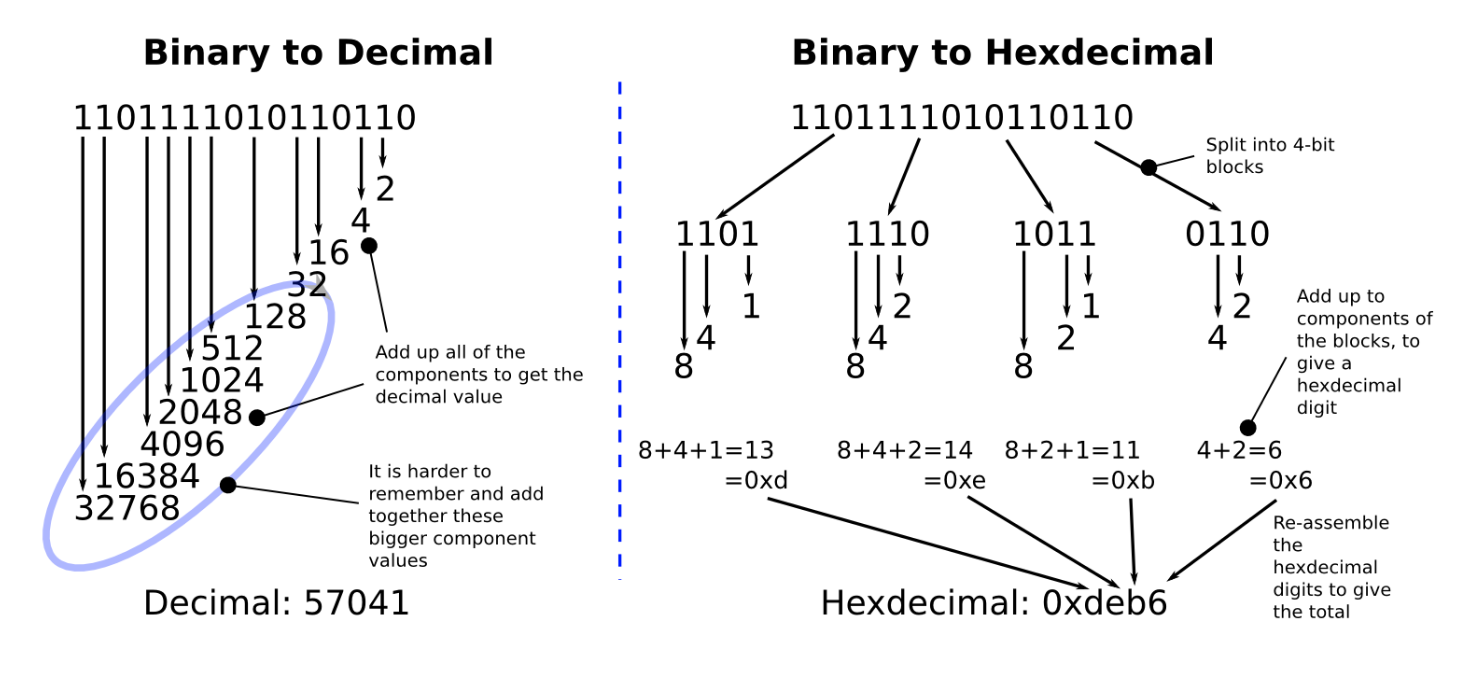
\includegraphics[width=0.8\textwidth]{binary_conversions}}
  \caption{\label{fig:2} Conversão de 1101111010110110 para decimal and hexadecimal} 
\end{figure}

O presente capítulo constituiu-se em apresentar conteúdos básicos e essencias para possibilitar a compreensão do funcionamento de computadores clássicos. Conteúdos que foram compreendidos a partir do desenvolvimento de um \href{https://github.com/gzsig/zsig-OS}{sistema operacional} simples que passa por todas as etapas essências do processo de ``boot'' do state of art de computadores clássicos: ligando em `modo real de 16 bits', transferindo-se para `modo protegido de 32 bits' e `gerencia interrupções'.

Tendo o entendimento avançado sobre a computação clássica, podemos avançar para a próxima geração: computadores quânticos.
\newpage

  \section{Computação Quântica} 
\label{quantum_comp}

A computação quântica é uma abordagem inovadora quando se trata de processamento de dados na computação. Neste capítulo é apresentado uma breve recuperação da história da área, assim bem como seus conceitos basilares e até mesmo os previstos impactos que acompanharão a funcionalidade desta inovação. Ainda, estudos adicionais estão sendo feitos a fim de complementar o capítulo para a entrega do relatório final.

\subsection{História}
Como proposto pelo cronograma desse estudo\footnote{página \pageref{updated_timeline} tabela \ref{updated_timeline}}, o presente capítulo, a ser desenvolvido no decorrer do segundo semestre, adentrará o desenvolvimento da Computação Quântica assim como a descrição de sua arquitetura – tema de extrema atualidade. O capítulo partirá do estudo de Alexander Holevo, publicado em 1973, que obteve como resultado o conhecido "teorema de Holevo"\footnote{um importante teorema limitativo na computação quântica, um campo interdisciplinar da física e da ciência da computação. Às vezes chamado de limite de Holevo, uma vez que estabelece um limite superior para a quantidade de informação que pode ser conhecida sobre um estado quântico.} – marco da computação quântica –, perpassando pela sua história até os dias atuais. Assim, poderemos compreender as implicações dos avanços em relação aos computadores quânticos, que como mencionado pelo artigo “Google claims its quantum computer can do the impossible in 200 seconds” \cite{16} já consegue resolver um problema, que levaria 10.000 anos para ser solucionado pelo supercomputador (clássico) mais rápido do mundo, em 200 segundos.

A Computação Quântica apresenta um novo horizonte de possibilidades no âmbito da computação. Acredita-se que os computadores quânticos sejam capazes de resolver certos problemas computacionais, como a factoração de inteiros – que é a base da criptografia RSA assunto aprofundado no capítulo \ref{criptography} –, substancialmente mais rápido do que os computadores clássicos.

A abordagem da computação quântica em relação à computação clássica se refere a como os dados são representados. Enquanto na computação clássica cara bit é um estado possível entre ``0'' e ``1'', já na computação quântica essa representação é probabilística, onde o dado pode estar em ambos estados ao mesmo tempo. Esse comportamento permite uma nova forma de nomear o bit, o \textbf{qubit}.

\subsection{Qubits}
\label{qubits}
Na mecânica quântica, uma partícula pode assumir dois estados ao mesmo tempo, o que é chamado de superposição. Ao aplicar este conceito à computação, temos uma partícula como um bit \footnote{melhor explicado na página \pageref{bits}} quântico, qubit (um bit quântico, unidade básica de informação em um computador quântico) que poderia retornar três posições: ligado (1), desligado (0), ou uma superposição de ambos, 1 e 0. Assim, um qubit pode comportar dois valores de uma vez; dois qubits quatro valores; e assim por diante. Isso significa que uma quantidade pequena de átomos pode comportar valores muito maiores do que os transístores de um computador binário, sendo mais eficiente. Um exemplo disto, seria o computador quântico da Google, que segundo WHYTE \cite{20}, realizou um cálculo de um problema em 200 segundos, que poderia demorar cerca de 10.000 anos para ser resolvido pelo melhor supercomputador existente, alcançando assim, a supremacia quântica.

\vspace{1cm}
\begin{figure}[H] \centering 
  \makebox[\textwidth][c]{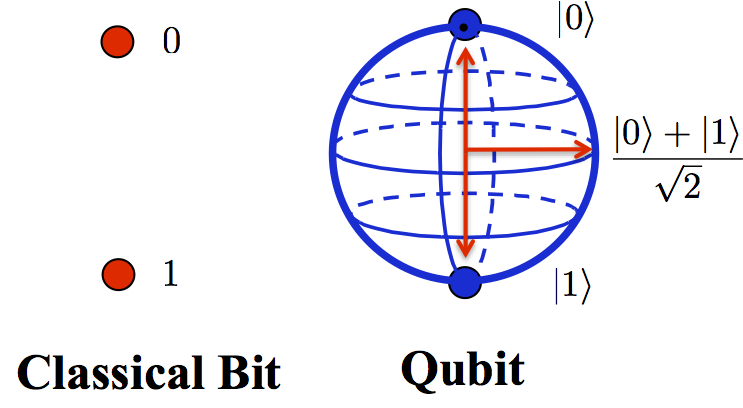
\includegraphics[width=0.5\textwidth]{bit_vs_qubit.png}}
  \caption{\label{bit_vs_qubit} A quantidade ilimitada de estados em que um qubit pode estar em um determinado momento é tradicionalmente representada em uma esfera onde Norte = 1 e Sul = 0. \href{https://www.autodesk.com}{autodesk.com}} 
\end{figure}

\subsection{Implementações}
Desde a década de 2000 as grandes empresas da computação vem se enfrentando na corrida por atingir a melhor arquitetura quântica funcional. Entre elas, destaca-se as duas grandes referencias no mercado da tecnologia: Google e IBM. Em 2019 a Google anunciou que havia atingido supremacia quântica como visto através do artigo: ``Quantum supremacy using a programmable superconducting processor'', \cite{17} coloca toda a sociedade às portas de um novo mundo, pois com esse poder computacional, problemas de otimização, que até então jamais seriam solucionados em tempo hábil, agora, estariam resolvidos em períodos mínimos de tempo.

Já a IBM, vem traçando a sua trajetória quântica desde 2016, lançando em maio de 2016 o IBM Q Experience, que continha um processador quântico de cinco qubit e um simulador de correspondência. Essa arquitetura, possibilitou que os usuários só interagissem por meio do compositor quântico, com um conjunto limitado de interações de dois qubit e um guia do usuário que assumiu experiência em álgebra linear. Em 2018 essa experiência teve significantes avanços, como exposto por Yuanhao Wang em seu artigo ``16-qubit IBM universal quantum computer can be fully entangled'', ``Os dispositivos backend atuais, da IBM incluem dois processadores com 5 qubits supercondutores sendo eles o ibmqx2 e o ibmqx4, um processador de 16 qubit, ibmqx5 e um processador de 20 qubit QS1\_1.'' \cite{18}, um grande avanço em apenas 4 anos. Atualmente, a empresa já vislumbra horizontes que pareciam muito distantes, anunciando que em 2023 terá um computador e David Nield – jornalista que escreve sobre ciência e tecnologia há mais de 20 anos tendo artigos publicados na Wired, Popular Science, The Guardian e Gizmodo – acredita que ``Com o IBM Quantum Condor planejado para 2023 - executando 1121 qubits, para ser exato - devemos começar a ver os computadores quânticos começarem a lidar com um número substancial de cálculos genuínos do mundo real, em vez de ficarem restritos a experimentos de laboratório.'' \cite{19}

\subsection{Dificuldades}
Apesar do avanços trazidos anteriormente, existem quatro principais dificuldades que impossibilitam o desenvolvimento e a escala de computadores quânticos no cenário atual: a qualidade do Qubit; implementação de algoritmos de correção de erros; o controle dos Qubits; e a grande quantidade de fios presentes na arquitetura.
Em relação à qualidade dos Qubits, a comunidade de estudiosos da computação quântica ainda não conseguiu chegar a um Qubit capaz de gerar instruções úteis em grande escala. Atualmente os poucos qubits nos computadores quânticos baseados em nuvem não são bons o suficiente para sistemas de grande escala,gerando erros ao executar operações entre dois qubits a uma taxa muito maior do que o necessário para se calcular com eficácia. Assim, após um certo número de instruções ou operações, os qubits atuaisproduzem uma resposta errada quando executamos cálculos, tendo a possibilidade do resultado obtido  ser indistinguível do ruído.
Uma vez que os qubits não são bons o suficiente para a escala em que precisamos que eles operem, precisamos implementar algoritmos de correção de erros que verifiquem e corrijam os erros de qubit aleatórios à medida que ocorrem. Esses são conjuntos de instruções complexos que utilizam muitos qubits físicos para estender efetivamente o tempo de vida das informações no sistema. A correção de erros ainda não foi comprovada em escala para a computação quântica, mas é uma área prioritária de pesquisa, a qual é considerada pré-requisito para um sistema quântico comercial em escala real.
Controle de Qubit: Para implementar algoritmos complexos, incluindo esquemas de correção de erros, é necessário provar a possibilidade controlar vários qubits. Esse controle deve ter baixa latência - da ordem de 10 de nanossegundos e deve vir de circuitos de controle de feedback adaptativo baseados em CMOS\footnote{abreviação de "Complementary Metal Oxide Semiconductor". O CMOS é uma pequena área de memória volátil, alimentada por uma bateria, que é usada para gravar as configurações do Setup da placa mãe.}. Este é um argumento semelhante ao apresentado no artigo do IEEE Spectrum , ``The Case Against Quantum Computing''. No entanto, embora seja assustador, existem motivos para acreditar que não é impossível.
Por fim, precisamos abordar o “fan-out” - ou como aumentar o número de qubits em um chip quântico. Hoje, exigimos vários fios de controle, ou vários lasers, para criar cada qubit. É difícil acreditar a viabilidade de construir um chip de um milhão de qubit com muitos milhões de fios conectando-se à placa de circuito ou saindo da câmara de medição criogênica. Na verdade, a indústria de semicondutores reconheceu esse problema em meados da década de 1960 e o chamou de Regra de Rent.

Além das dificuldades de implementações e apesar das diversas iniciativas, o maior problema repousa em como se provar que a computação quântica foi alcançada, pois para isso, um problema que poderia ser resolvido em 50 bilhões de anos de fato precisa ser solucionado.

\subsection{Impactos}
Avançando alguns anos para o futuro, nos situando em um tempo na qual os problemas apresentados anteriormente já foram e resolvidos, tendo um computador quântico funcional, é possível podemos imaginar os impactos que acompanharão essa nova tecnologia. Com a capacidade de “multitarefas” da computação quântica, diversos problemas computacionais cuja complexidade é NP poderão ser resolvidos em tempo hábil, o quê poderá se tornar um problema para áreas que fazem uso desta característica como artifício de trabalho, como a criptografia, temática abordada no capítulo \ref{criptography}.
Além da criptografia, há diversas outras frentes de trabalho que serão impactadas pela computação quântica e que poderão impactar outras soluções que são empregadas em problemas do cotidiano, dos quais a sociedade faz uso e que tal inovação poderá pôr por terra toda a engenhosidade da solução, aprofundado pelo capítulo \ref{social_impacts}, que trata sobre a temática de forma mais ampla.


\newpage
  \section{Computador} 
\textbf{Ressalva: }
\textit{Esse capítulo foi reservado para descrever o passo a passo de como desenvolver um computador clássico apenas com portas logicas simples. Devido a alguns problemas esclarecidos na seção \ref{problems} e tendo em vista que o protótipo ainda não foi desenvolvido, é proposto que essa parte seja adiada para um possível futuro trabalho.}
\newline
\newline
Construir um computador parece uma tarefa complicada e ousada. Porém, uma CPU\footnote{CPU é a sigla para Central Process Unit, ou Unidade Central de Processamento. É o principal item de hardware do computador, que também é conhecido como processador, essa é a parte responsável por calcular e realizar tarefas determinadas pelo usuário.} é bastante simples em operação depois que os fundamentos por trás de todos os seus processos são compreendidos. Desta maneira, este capítulo destina-se em explicar o passo a passo para que qualquer pessoa interessada, seja capaz de construir seu próprio computador e obter o conhecimento que acompanha o processo.

\subsection{Módulos}
Para facilitar a compreensão, e também o desenvolvimento do computador, este capítulo será dividido em alguns subcapítulos, em que cada qual abordará sobre uma parte do computador.

\subsubsection{Clock}
O clock do computador é uma parte essencial para o seu funcionamento. Este tem a função de sincronizar todas as operações. A ação mais rápida que o computador consegue executar é equivalente a uma vibração do seu clock.

\subsubsection{Registers}
A maioria das CPUs possuem vários registradores que armazenam pequenas quantidades de dados processados pela CPU. Em nossa CPU de breadboard, criaremos três registradores de 8 bits: A, B e IR. Os registradores A e B são para uso geral. Já o IR (instruction register), apesar de funcionar da mesma forma, é usado para armazenar a instrução atual que está sendo executada.

\subsubsection{Arithmetic logic unit (ALU)}
A parte da unidade lógica aritmética (ALU) de uma CPU geralmente é capaz de executar várias operações aritméticas, bit a bit e de comparação em números binários. Em nossa CPU de breadboard, a ALU pode apenas adicionar e subtrair. Ele está conectado aos registradores A e B e gera a soma de A + B ou a diferença de A-B.

\subsubsection{Random access memory (RAM)}
A memória de acesso aleatório (RAM) armazena o programa que o computador está executando, bem como todos os dados que o programa precisa. Nosso computador de breadboard utiliza endereços de 4 bits, o que significa que ele terá apenas 16 bytes de RAM, limitando o tamanho e a complexidade dos programas que poderá executar.

\subsubsection{Program counter}
O contador do programa (Program counter) conta em binário para acompanhar qual instrução o computador está executando no momento.

\subsubsection{Output register}
O registrador de saída é semelhante a qualquer outro registrador (como os registradores A e B), exceto que, em vez de exibir seu conteúdo em binário em 8 LEDs, ele exibe seu conteúdo de forma decimal em um display de 7 segmentos, o que requer uma lógica complexa.

\subsubsection{CPU control logic}
A lógica de controle é o coração da CPU. É o que define os códigos de operação (opcode) que o processador reconhece e o que acontece quando ele executa cada instrução.

\subsubsection{Materiais Necessários}

\newpage



  \section{Simulador} 
  \section{Criptografia}
Conforme definido por Bruce Schneier \textit{``The art and science of keeping messages secure is cryptography […].''} \cite{13} Embora a criptografia seja considerada fundamental em nossas vidas digitais, ela não está especificamente relacionada à computação. A criptografia existe em diversas formas há milênios.

Na segurança cibernética, há uma série de preocupações quando se trata de dados. Isso inclui confidencialidade, integridade, disponibilidade e não repúdio.

\textbf{A confidencialidade} significa que nossos dados não podem ser acessados / lidos por usuários não autorizados.

\textbf{A integridade} do dado diz respeito à originalidade na qual os dados chegam à nós, estando 100\% intactos, sem terem sido modificados - seja por um ator malicioso, perda de dados ou por algum outro fator. 

\textbf{A disponibilidade} se refere à acessibilidade dos dados quando necessário.

Examinaremos as várias formas de criptografia digital e como elas podem nos ajudar a alcançar os três objetivos listados acima. Quando falamos de criptografia digital, geralmente nos referimos a uma das seguintes criptografias, que serão melhor explicadas e exemplificadas na própria sessão.

\begin{enumerate}
  \item Criptografia simétrica
  \item Criptografia assimétrica
  \item Funções de hash
\end{enumerate}

Esses conceitos serão explicados e exemplificados na próxima secção.

É temido que os computadores quânticos sejam capazes de decifrar certos códigos usados para enviar mensagens seguras. Os códigos em questão criptografam dados usando funções matemáticas de ``trapdoor'' que funcionam facilmente em uma direção, mas não em outra. Isso facilita a criptografia de dados, mas a decodificação é extremamente difícil sem a ajuda de uma chave especial.

Esses sistemas de criptografia nunca foram inquebráveis, sua segurança se baseia na enorme quantidade de tempo que um computador clássico levaria para fazer o trabalho. Os métodos modernos de criptografia são projetados especificamente para que a decodificação demore tanto tempo de forma a serem praticamente inquebráveis.

No entanto, os computadores quânticos mudaram esse pensamento. Essas máquinas são muito mais poderosas que os computadores clássicos, tornando possível o rompimento desses códigos com facilidade, já que realizam contas matemáticas de forma mais eficiente e significativamente mais rápido que os computadores clássicos.

\subsection{Conceitos básicos de criptografia}
Antes de mergulharmos nisso: o que exatamente queremos dizer com "criptografia"? Criptografar e descriptografar são normalmente usadas para significar criptografia e decifração, respectivamente; para simplificar, criptografar uma mensagem significa torná-la ilegível para partes não autorizadas usando uma cifra (o método específico para fazer isso). Descriptografar a mensagem significa reverter o processo e tornar os dados legíveis mais uma vez.

\subsubsection{Criptografia simétrica}
Para criptografar e descriptografar corretamente nossos dados, precisamos dos dados e de uma chave (que determina a saída da nossa cifra).
Com a criptografia simétrica, a chave usada para criptografar e descriptografar dados é a mesma.

\subsubsection{Criptografia assimétrica}
O problema da criptografia simétrica é o seguinte: E se eu precisar enviar dados com segurança em um ambiente hostil, como a Internet? Se a mesma chave for usada para criptografar e descriptografar dados, primeiro eu precisaria enviar a chave de descriptografia para estabelecer uma conexão segura. Mas isso significa que estou enviando a chave por uma conexão insegura, o que significa que a chave pode ser interceptada e usada por terceiros! Como contornar isso? 

Para exemplificar, usaremos um cadeado que possui três estados: A (bloqueado), B (desbloqueado) e C (bloqueado).
E tem duas chaves distintas. A primeiro pode girar apenas no sentido horário (de A a B a C) e a segunda pode girar apenas no sentido anti-horário (de C a B a A).

Ao criptografar uma mensagem, o usuário pega a primeira chave e guarda para si mesmo. Essa chave, sua chave "privada" - porque apenas ele a possui.

A segunda chave, sua chave ``pública'': Pode ser distribuida para qualquer pessoa. Assim, o usuário tem sua chave privada que pode mudar de A para B para C. E todo os outros tem sua chave pública que pode mudar de C para B para A.

Colocando isso em prática, imagine que você queira enviar um documento privado para o usuario. Você coloca o documento na caixa e usa uma cópia da chave pública dele para bloqueá-lo. Lembre-se de que a chave pública dele gira apenas no sentido anti-horário, e você a coloca na posição A. Agora a caixa está bloqueada. A única chave que pode passar de A para B é a chave privada, a que ele guardou para si.

\subsubsection{Funções de hash}
Uma função de hash, diferente da criptografia simétrica / assimétrica, é uma função unidirecional. Você pode criar um hash a partir de alguns dados, mas não há como reverter o processo. Como tal, não é uma maneira útil de armazenar dados, mas é uma maneira útil de verificar a integridade de alguns dados.
Uma função de hash recebe alguns dados como entrada e gera uma string aparentemente aleatória (mas nem tanto) que sempre terá o mesmo comprimento. Uma função de hash ideal cria valores exclusivos para diferentes entradas. A mesma entrada exata sempre produzirá exatamente o mesmo hash - e é por isso que podemos usá-la para verificar a integridade dos dados.

\subsection{Rivest Shamir Adleman – RSA Criando chave publica e privada}

% \begin{algorithm}[H]
%   \SetAlgoLined
%   \KwResult{Write here the result }
%    $p\prime$
%    \newline
%    $q\prime$
%    \newline
%    $n = p * q$
%    \newline
%    $\Phi(n)=(p-1)(q-1)$
%    \newline
%    initialization\;
%    \While{While condition}{
%     instructions\;
%     \eIf{condition}{
%      instructions1\;
%      instructions2\;
%      }{
%      instructions3\;
%     }
%    }
%    \caption{How to write algorithms}
%   \end{algorithm}

\vspace{1cm}
\begin{longtable}{ |p{6cm}|| p{8cm}|  }
  \hline
  \multicolumn{2}{|c|}{RSA – Cryptosystem} \\
  \hline
    Descrição & matemática\\
  \hline
    Escolher dois números primos & 
    \[p=2\] \[q=7\]\\
  \hline
    Produto dos números escolhidos & 
    \[n=14\]\\
  \hline
    função Phi 
    \[\Phi(n)=(p-1)(q-1)\] & 
    \[\Phi(14)=(7-1)(2-1)\]
    \[\Phi(14)=(6)(1)\]
    \[\Phi(14)=6\]
    \[Coprimos\: de\: 14:\: 1, 3, 5, 9, 11, 13\]\\
  \hline
    Escolher o numero e `encryption'
    \begin{itemize}
      \item $1 < e < \Phi(n)$
      \item $coprimo\: de: n\: e\: \Phi(n)$
    \end{itemize} &
    \[Coprimos\: de\: 14:\: 1, 3, 5, 9, 11, 13\]
    \[Coprimos\: de\: 6:\: 1, 5\]
    \[Menor\: que\: 6\: e\: coprimo\: de\: 14\: e\: de\: 6: 5\]
    \[e = 5\]\\
  \hline
    Chave publica & 
    \[(5, 14)\]\\
  \hline
  Escolher o numero d `decryption'
    \begin{itemize}
      \item $d * e (mod \Phi(n)) = 1$
    \end{itemize} & 
    \[d * 5 (mod 6) = 1\]
    \[5*d = 5, 10, 15, 20, 25 \dots 55\]
    \[5*1 (mod 6) = 5\]
    \[5*2 (mod 6) = 4\]
    \[5*3 (mod 6) = 3\]
    \[5*4 (mod 6) = 2\]
    \[5*5 (mod 6) = 1\]
    \[5*6 (mod 6) = 0\]
    \[ \dots \]
    \[5*11 (mod 6) = 1\] \\
  \hline
  Chave privada & 
  \[(11, 14)\]\\
  \hline
  \caption{Passo a passo para gerar par de chaves}
  \label{table:3}
\end{longtable}

\vspace{1cm}
\begin{longtable}{ |p{6cm}|| p{8cm}|  }
  \hline
  \multicolumn{2}{|c|}{RSA – Cryptosystem} \\
  \hline
    Descrição & matemática\\
  \hline
    Criptografar \newline
    Chave publica: $(5, 14)$ \newline
    mensagem: ``B'' 
    \[A \to 1\]
    \[B \to 2\]
    \[C \to 3\]
    \[D \to 4\] & 
    \[2^5(mod 14)\]
    \[32(mod 14)\]
    \[4(mod 14)\]
    Mensagem criptografada: 4 $\to$ D\\
  \hline
    Descriptografar \newline
    Chave privada: $(11, 14)$ \newline
    mensagem: ``D'' 
    \[A \to 1\]
    \[B \to 2\]
    \[C \to 3\]
    \[D \to 4\] & 
    \[4^{11}(mod 14)\]
    \[4194304(mod 14)\]
    \[2(mod 14)\]
    Mensagem original: 2 $\to$ B\\
  \hline
  \caption{Como criptografar e decifrar}
  \label{table:4}
\end{longtable}

\subsection{Criptografia aplicada computação clássica}
\subsection{Criptografia aplicada computação quântica}
\newpage


  \section{Próximos passos}
\label{next_steps}
\subsection{Cronograma}
\vspace{1cm}
\begin{longtable}{ |p{2.5cm}||p{0.60cm}|p{0.60cm}|p{0.60cm}|p{0.60cm}|p{0.60cm}|p{0.60cm}|p{0.60cm}|p{0.60cm}|p{0.60cm}|p{0.60cm}|p{0.60cm}|p{0.60cm}|p{0.60cm}|  }
  \hline
  \multirow{2}{*}{Etapas} & 
  \multicolumn{11}{|c|}{2020} & 
  \multicolumn{2}{|c|}{2021} \\
        &
    fev &
    mar &
    abr &
    mai &
    jun &
    jul &
    ago &
    set &
    out &
    nov &
    dez &
    jan &
    fev \\
  \hline
  Clássica & 
  \multicolumn{2}{|c|}{\cellcolor{blue!25}} & 
  & & & & & & & & & & \\
  \hline
  Quântico & 
  \multicolumn{2}{|c|}{\cellcolor{blue!25}} & 
  & & & & & & & & & & \\
  \hline
  Protótipo & &
  \multicolumn{4}{|c|}{\cellcolor{blue!25}} & 
  & & & & & & & \\
  \hline
  Entrega Parcial & & & &
  \multicolumn{5}{|c|}{\cellcolor{blue!25}} & 
  & & & & \\
  \hline
  Comparação & & & & & &
  \multicolumn{2}{|c|}{\cellcolor{blue!25}} & 
  & & & & & \\
  \hline
  Web App & &
  \multicolumn{8}{|c|}{\cellcolor{blue!25}} & 
  & & & \\
  \hline
  Impacto Social & & & & & & & &
  \multicolumn{4}{|c|}{\cellcolor{blue!25}} & 
  & \\
  \hline
  Entrega Final & & & & & & &
  \multicolumn{7}{|c|}{\cellcolor{blue!25}} \\
  \hline
  \caption{Cronograma original}
  \label{original_timeline}
\end{longtable}
\vspace{1cm}

Acima está uma réplica do cronograma originalmente proposto para este projeto. Na tabela a seguir está mesmo cronograma porém com algumas alterações pontuais:

Justificativa de cada alteração:
\begin{enumerate}
  \item \textbf{O projeto não começou em fevereiro de 2020} pois foi aprovado com ressalvas pela banca, assim esse mês foi dedicado ao aprimoramento da proposta.
  \item \textbf{O projeto foi separado em duas grandes partes} 2020.1 foi voltado a computação clássica, e o plano é que 2020.2 será focada em computação quântica. Essa mudança relevante se dá pelo entendimento de que uma pesquisa de apenas dois meses no ramo da computação se tornaria algo raso e os principais conceitos não seriam abordados com a devida intensidade.
  \item \textbf{O não desenvolvimento do protótipo} ocorreu pelo atraso na compra dos materiais.
  \item \textbf{A inclusão do Sistema Operacional e Simulador 24bits} foi uma forma de manter a metodologia \textit{``Project Based Learning''} para o aprendizado na área de computação clássica sem ter os materiais desejados em mãos.
\end{enumerate}

\vspace{1cm}
\begin{longtable}{ |p{2.5cm}||p{0.60cm}|p{0.60cm}|p{0.60cm}|p{0.60cm}|p{0.60cm}|p{0.60cm}|p{0.60cm}|p{0.60cm}|p{0.60cm}|p{0.60cm}|p{0.60cm}|p{0.60cm}|p{0.60cm}|  }
  \hline
  \multirow{2}{*}{Etapas} & 
  \multicolumn{11}{|c|}{2020} & 
  \multicolumn{2}{|c|}{2021} \\
        &
    fev &
    mar &
    abr &
    mai &
    jun &
    jul &
    ago &
    set &
    out &
    nov &
    dez &
    jan &
    fev \\
  \hline
  Clássica & &
  \multicolumn{6}{|c|}{\cellcolor{green!25}} & 
  & & & & & \\
  \hline
  Quântico & &
  \multicolumn{1}{|c|}{\cellcolor{green!25}} & 
  & & & &
  \multicolumn{2}{|c|}{\cellcolor{green!25}} & 
  \multicolumn{4}{|c|}{\cellcolor{blue!25}} & 
  \\
  \hline
  Protótipo & & & & &
  \multicolumn{1}{|c|}{\cellcolor{green!25}} & 
  & & & & & & & \\
  \hline
  Entrega Parcial & & & &
  \multicolumn{5}{|c|}{\cellcolor{green!25}} & 
  & & & & \\
  \hline
  Comparação & & & & & & & & & &
  \multicolumn{2}{|c|}{\cellcolor{blue!25}} & 
  & \\
  \hline
  Códigos & &
  \multicolumn{7}{|c|}{\cellcolor{green!25}} & 
  \multicolumn{4}{|c|}{\cellcolor{blue!25}} & 
  \\
  \hline
  Sistema Operacional & & &
  \multicolumn{5}{|c|}{\cellcolor{green!25}} & 
  & & & & & 
  \\
  \hline
  Simulador 24bits & & &
  \multicolumn{5}{|c|}{\cellcolor{green!25}} & 
  & & & & & 
  \\
  \hline
  Criptografia didática & & & & &
  \multicolumn{2}{|c|}{\cellcolor{green!25}} & 
  & & 
  \multicolumn{3}{|c|}{\cellcolor{blue!25}} & 
  &
  \\
  \hline
  Impacto Social & & & & & &
  \multicolumn{2}{|c|}{\cellcolor{green!25}} & 
  & &
  \multicolumn{2}{|c|}{\cellcolor{blue!25}} & 
  & \\
  \hline
  Entrega Final & & & & & & &
  \multicolumn{2}{|c|}{\cellcolor{green!25}} & 
  \multicolumn{5}{|c|}{\cellcolor{blue!25}} \\
  \hline
  \caption{Cronograma atualizado}
  \label{updated_timeline}
\end{longtable}
\vspace{1cm}

\subsection{Ajustes e correções possíveis no projeto}
% \label{problems}
Devido a pandemia e principalmente ao atraso não previsto de quatro meses da compra dos materiais para o desenvolvimento do protótipo, este, que estava no cronograma de 2020.1 ainda não foi finalizado, apesar de já iniciado. Ainda, há preocupações com relação a essa finalização, devido ao grande esforço ainda necessário.
Além disso, um estudo já foi feito sobre computação quântica, ainda não em definitivo, já que se trata de um relatório parcial, conforme evidenciado pelo Capítulo \ref{computer}. Há preocupações, também, com relação ao prazo para a implementação do simulador de computação quântica, dado que ainda precisa ser melhor estudado. 


\newpage

  \section{Impactos sociais}
\label{social_impacts}
O avanço da computação quântica seguramente afetará o mundo atual de diversas formas. Entre elas, impactando temáticas como: privacidade; política; otimização de logística e melhor tomada de decisão por máquina.

O principal motivo é resultado do desempenho mais ágil que computadores quânticos tem quando são comparados aos mais modernos da atualidade – clássicos – podem facilmente fazer o que parece ser uma tarefa impossível para computadores clássicos. Eles conseguem resolver e quebrar algoritmos de criptografia que protegem os dados de um usuário e a infraestrutura da Internet, além de otimizar melhores caminhos para logística e sempre tomarem a melhor decisão.

Em outubro de 2019, o Google revelou sua bem-sucedida experiência “Quantum Supremacy”, alegando que um problema particularmente difícil havia sido resolvido em 200 segundos 
 \cite{15}.

\subsection{Criptografia \& Privacidade}
A criptografia atual é baseada em matemática e decodificação, sendo essa é uma tarefa bastante complicada para computadores clássicos. No entanto,os computadores quânticos a executam com grande facilidade. O algoritmo de fatoração de Shor\footnote{Um algoritmo de computador quântico de tempo polinomial para fatoração de número inteiro. Informalmente, resolve o seguinte problema: Dado um número inteiro, encontre seus fatores primos. Foi inventado em 1994 pelo matemático americano Peter Shor} é de particular importância para essa temática, pois significa que a criptografia de chave pública pode ser facilmente quebrada. Tendo em vista a “falha” na criptografia, o tema de privacidade vem à tona, sendo abordado no atual capítulo como esse fenômeno se comporta em três situações: negócios privados, transações e política.

\subsubsection{Negócios privados}
Empresas modernas de forma geral armazenam e gerenciam a maioria de suas informações pessoais e confidenciais de forma online, em uma nuvem com conexão ininterrupta à web. Assim, é quase impossível conduzir tais informações de forma a evitar que os dados caiam nas mãos de terceiros. Por  esse motivo a criptografia está sendo incorporada aos planos de segurança de dados em nuvem de empresas, mantendo seus dados privados e seguros, independentemente de sua localização. 

De acordo com o estudo “Data Breach” da IBM em 2018, o custo para cobrir uma violação de dados média é de US \$ 3,86 milhões. Estima-se que este custo deve aumentar 6,4\% em 2019, com a probabilidade de uma violação recorrente nos próximos dois anos, chegando a aumentar 27,9\%. Essa estatística por si só é suficiente para as empresas considerarem maneiras de otimizar suas medidas de segurança,que garantam a proteção ideal dos dados de suas empresas.

\subsubsection{Transações}
No modelo atual, as transações acontecem de forma criptografada. A melhor maneira de essa temática é através da internet. Qualquer endereço que começe com “https://” é criptografado, o que significa que ninguém, a não ser quem acessa a página e o servidor tem acesso aos conteúdos transacionados. Com alguns níveis de abstração, esse processo também acorre com transações bancarias, em que apenas o dono da conta consegue visualizar o saldo presente na conta e fazer operações. Já no modelo futuro, quando os computadores quânticos tiverem a estabilidade que os computadores clássicos tem hoje, todos esses dados e acessos serão públicos. Este é um pensamento assustador, porém muito realista.

Um dos métodos mais eficazes para proteger dados é por meio de criptografia. Assim como se tranca as portas de espaços importantes em empresas para impedir uma invasão, é preciso fazer o mesmo com os dados por meio de criptografia. Em vez de trancar uma porta física, a criptografia coloca algoritmos baseados em algoritmos matemáticos para protegê-los de hackers.


\subsubsection{Política}
Com o avanço da computação quântica, uma realidade de perda de privacidade se aproxima rapidamente. Isso afetará involuntariamente a política interna e externa de muitos países. 

No escopo interno, as implicações da perda da privacidade das comunicações são preocupações importantes para os direitos humanos, por exemplo, em países onde regimes políticos opressores encontram interesse em manter a ficção de que todos os sujeitos concordam com seus pontos de vista. Com esses avanços, será possível usar medidas de vigilância secretas para monitorar dissidentes e rastrear as atividades de pessoas consideradas suspeitas que poderia sufocar a dissidência política, um objetivo que tem sido aspirado muitas vezes historicamente, mas nunca antes alcançado.  Assim, é claramente uma tentação para os governos realizar esse tipo de vigilância. O problema potencial não está isolado dos regimes opressores, mas provavelmente aparecerá de uma forma diferente (ilegal) nas democracias tradicionais, onde os cidadãos tradicionalmente atribuem um alto valor à privacidade. As implicações são amplas e para as democracias menos seguras são consideravelmente mais sinistras.

No escopo externo,  há a questão da desigualdade de conhecimento – informações sigilosas poderão ser acessadas por outros países – e portanto, será possível aumentar o poder de barganha em meio as negociações de comercio e relações internacionais.

\subsection{Otimização}
A computação quântica permite a otimização em diversas áreas. Essas incluem busca de melhores caminhos – logística em tempo-hábil,  melhor tomada de decisão de forma não empírica, robótica – tomar SEMPRE a melhor decisão e vale pena enfrentar uma decisão computacional?

\subsubsection{Busca de melhores caminhos – logística em tempo-hábil}
O problema de encontrar o caminho mais curto entre dois pontos em um grá- fico ponderado é antigo. A questão de quais algoritmos clássicos podem ser acelerados pela computação quântica é, obviamente, muito interessante. No mo- mento, existem apenas algumas técnicas gerais conhecidas no campo da computação quântica e a descoberta de novos problemas, passíveis de acelerações quânticas, é uma alta prioridade. Uma dessas técnicas gerais de soluções de problemas por meio da computação quântica foi considerada no Trabalho de Heiligman  \cite{21}.

No caso clássico, o trabalho total para o o algoritmo é max $ (O(kn^2),  O(n^2)) = O(n^2) $  qual é minimizado tomando $ k = 1 $ , portanto $ W classico=O(n^2) $

No caso quântico, a situação é um pouco diferente. O trabalho total na primeira etapa é apenas o máximo de o trabalho nas próximas duas etapas, desde o trabalho na primeira etapa é sempre dominada por esses outros fatores de trabalho. O trabalho total é, portanto, max$ (O(k^1/2 n^3/2), O(k^1/2 n^2)) $

e para minimizar isso, o parâmetro $ k $ deve ser escolhido para tornar esses dois fatores de trabalho iguais. Definição $ k^1/2 n^3/2= k^-1/2 n^2 $ dá $ k = n^1/2 $ e portanto $W quantico = O(n^7/4) $

Na verdade, isso é uma melhoria em relação ao clássico fator de trabalho de $ n^2 $

\subsubsection{melhor tomada de decisão de forma não empírica}
\subsubsection{Robótica – tomar SEMPRE a melhor decisão}
\subsubsection{Vale pena enfrentar uma decisão computacional?}

\subsection{Considerações finais - incompleto}
Assim, o impacto que o avanço da física quântica aplicada a computação terá na criptografia, supera as barreiras técnicas e afeta de maneira irreversível diversas outras áreas. Para mitigar os danos gerados por esse avanço, em paralelo estão sendo feitos estudos que avançam na área da criptografia quântica. Mas esses ainda não apresentam soluções aplicáveis e viáveis em tempo hábil.

\newpage
  \section{Conclusões}
Nesse capítulo serão colocadas as conclusões ao final do projeto.
\subsection{Perspectivas}

\newpage
  \section{Apêndice A – Sistema Operacional}
\label{apendeceA}

Além do trabalho desenvolvido no projeto, um protótipo de sistema operacional foi feito.

Esse protótipo contempla: inicialização.

 Conteúdos que foram compreendidos a partir do desenvolvimento de um \href{https://github.com/gzsig/zsig-OS}{sistema operacional} simples que passa por todas as etapas essenciais do processo de ``boot'' – ilustrado na figura a baixo – \textit{state-of-the-art} de computadores clássicos: ligando em `modo real de 16 bits', carregando o kernel\footnote{Uma parte integrante de qualquer sistema operacional. Que se constitui em um programa com controle completo sobre tudo no sistema.}, transferindo-se para `modo protegido de 32 bits' e `gerenciando interrupções'.

\vspace{1cm}
\begin{figure}[H] \centering 
  \makebox[\textwidth][c]{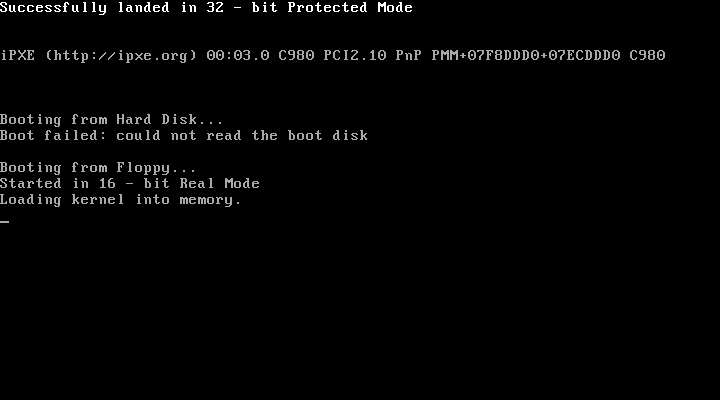
\includegraphics[width=0.8\textwidth]{zsig_OS_boot.png}}
  \caption{\label{zsig_OS_boot} Processo de boot} 
\end{figure}

  \newpage
  \bibliography{referencias}
\end{document}
